\documentclass[10pt,t]{beamer}


\setbeamersize{text margin left=10pt,text margin right=10pt}
\usetheme{lehigh}

\usefonttheme{professionalfonts}
\usefonttheme{serif}

%\usepackage{pgf,pgfarrows,pgfnodes,pgfautomata,pgfheaps,pgfshade}
%\usepackage{amsmath,amssymb,amsfonts,subfigure,pifont}
\usepackage{multirow,multicol}
%\usepackage{tabularx}
%\usepackage{booktabs}
\usepackage{colortbl}
\usepackage{algorithm,algpseudocode}
%\usepackage{etex}
\usepackage{fancyvrb,listings}

\definecolor{dkgreen}{rgb}{0,0.6,0}
\definecolor{grey}{rgb}{0.5,0.5,0.5}
\definecolor{mauve}{rgb}{0.58,0,0.82} 
\lstset{%
language=bash,                % the language of the code
%basicstyle=\footnotesize,           % the size of the fonts that are used for the code
basicstyle=\fontsize{4.5}{5.5}\selectfont\ttfamily,
showspaces=false,               % show spaces adding particular underscores
showstringspaces=false,         % underline spaces within strings
showtabs=false,                 % show tabs within strings adding particular underscores
%frame=single,                   % adds a frame around the code
%rulecolor=\color{black},        % if not set, the frame-color may be changed on line-breaks within not-black text (e.g. comments (green here))
tabsize=2,                      % sets default tabsize to 2 spaces
%captionpos=b,                   % sets the caption-position to bottom
breaklines=true,                % sets automatic line breaking
breakatwhitespace=false,        % sets if automatic breaks should only happen at whitespace
%title=\lstname,                   % show the filename of files included with \lstinputlisting;
% also try caption instead of title
keywordstyle=\color{blue},          % keyword style
commentstyle=\color{dkgreen},       % comment style
stringstyle=\color{mauve},         % string literal style
escapeinside={\%*}{*)},            % if you want to add LaTeX within your code
morekeywords={*,\dots,elif},              % if you want to add more keywords to the set
deletekeywords={\dots},              % if you want to delete keywords from the given language
%morecomment=[l]{//}
}
\lstset{%
language=csh,                % the language of the code
%basicstyle=\footnotesize,           % the size of the fonts that are used for the code
basicstyle=\fontsize{4.5}{5.5}\selectfont\ttfamily,
showspaces=false,               % show spaces adding particular underscores
showstringspaces=false,         % underline spaces within strings
showtabs=false,                 % show tabs within strings adding particular underscores
%frame=single,                   % adds a frame around the code
%rulecolor=\color{black},        % if not set, the frame-color may be changed on line-breaks within not-black text (e.g. comments (green here))
tabsize=2,                      % sets default tabsize to 2 spaces
captionpos=b,                   % sets the caption-position to bottom
breaklines=true,                % sets automatic line breaking
breakatwhitespace=false,        % sets if automatic breaks should only happen at whitespace
%title=\lstname,                   % show the filename of files included with \lstinputlisting;
% also try caption instead of title
keywordstyle=\color{blue},          % keyword style
commentstyle=\color{dkgreen},       % comment style
stringstyle=\color{mauve},         % string literal style
escapeinside={\%*}{*)},            % if you want to add LaTeX within your code
morekeywords={*,\dots,elif},              % if you want to add more keywords to the set
deletekeywords={\dots},              % if you want to delete keywords from the given language
%morecomment=[l]{//}
}
\lstdefinestyle{LINUX}
{
%    backgroundcolor=\color{black},
    basicstyle=\tiny\ttfamily,
%    keywordsstyle=\color{blue},
%    morekeywords={Tutorials,BASH,scripts},
%    literate={>}{{\textcolor{blue}{>}}}1
%         {/}{{\textcolor{blue}{/}}}1
%         {./}{{\textcolor{black}{./ }}}1
%         {~}{{\textcolor{blue}{\textasciitilde}}}1,
}

\lstdefinestyle{customc}{
  belowcaptionskip=1\baselineskip,
  breaklines=true,
  xleftmargin=\parindent,
  language=C,
  showstringspaces=false,
  basicstyle=\footnotesize\ttfamily,
  keywordstyle=\bfseries\color{green!40!black},
  commentstyle=\upshape\color{red!90!white},
  identifierstyle=\color{blue},
  stringstyle=\color{orange},
}
\lstdefinelanguage{OmpFortran}[]{Fortran}{
   rulesepcolor=\color{black},
   %
   extendedchars=true,
   %
   morecomment=[l] [\bfseries\color{red!90!white}]{!\$omp},
   morecomment=[l] [\bfseries\color{red!90!white}]{c\$omp},
   morecomment=[l] [\bfseries\color{red!90!white}]{*\$omp},
   morecomment=[l] [\bfseries\color{red!90!white}]{!\$acc},
   morecomment=[l] [\bfseries\color{red!90!white}]{c\$acc},
   morecomment=[l] [\bfseries\color{red!90!white}]{*\$acc},
}[comments]

\lstdefinelanguage{OmpC}[]{OmpFortran}{
   rulesepcolor=\color{black},
   %
   extendedchars=true,
   %
   morecomment=[l] [\bfseries\color{red!90!white}]{\#pragma\ omp},
   morecomment=[l] [\bfseries\color{red!90!white}]{\#pragma\ acc},
}[comments]

\lstset{escapechar=@,style=customc}
\lstset{literate=%
   *{0}{{{\color{blue}0}}}1
    {1}{{{\color{blue}1}}}1
    {2}{{{\color{blue}2}}}1
    {3}{{{\color{blue}3}}}1
    {4}{{{\color{blue}4}}}1
    {5}{{{\color{blue}5}}}1
    {6}{{{\color{blue}6}}}1
    {7}{{{\color{blue}7}}}1
    {8}{{{\color{blue}8}}}1
    {9}{{{\color{blue}9}}}1
}

\algrenewcommand\algorithmicfunction{\textbf{program}}
\algblockdefx[Program]{Program}{EndProgram}[1]{\textbf{program} \textsc{#1}}[1]{\textbf{end program} \textsc{#1}}
\algloopdefx[doloop]{Do}[1]{\textbf{do} #1}
\algcblockdefx[doloop]{If}{Do}{EndDo}
[1]{\textbf{do} #1}{\textbf{end do}}


\usepackage{tikz}
\usetikzlibrary{shapes,arrows,matrix}
\usetikzlibrary{calc}
\pgfdeclarelayer{background}
\pgfdeclarelayer{foreground}
\pgfsetlayers{background,main,foreground}
\usepackage[latin1]{inputenc}
\usepackage[english]{babel}
\usepackage{hyperref}
\usepackage[normalem]{ulem}
% \usepackage{movie15} 

                                                         
\usepackage{times}
\usepackage[T1]{fontenc}
\usepackage{graphicx}


\definecolor{DarkGreen}{rgb}{0.0,0.3,0.0}
\definecolor{Blue}{rgb}{0.0,0.0,0.8} 
\definecolor{dodgerblue}{rgb}{0.1,0.1,1.0}
\definecolor{indigo}{rgb}{0.41,0.1,0.0}
\definecolor{seagreen}{rgb}{0.1,1.0,0.1}
\DeclareSymbolFont{extraup}{U}{zavm}{m}{n}
%\DeclareMathSymbol{\vardiamond}{\mathalpha}{extraup}{87}
\newcommand{\cmark}{\ding{51}}
\newcommand{\xmark}{\ding{55}}
\newcommand{\smark}{\ding{77}}
\newcommand*\vardiamond{\textcolor{lubrown}{%
  \ensuremath{\blacklozenge}}}
\newcommand*\up{\textcolor{green}{%
  \ensuremath{\blacktriangle}}}
\newcommand*\down{\textcolor{red}{%
  \ensuremath{\blacktriangledown}}}
\newcommand*\const{\textcolor{darkgray}%
  {\textbf{--}}}
\newcommand*\enter{\tikz[baseline=-0.5ex] \draw[<-] (0,0) -| (0.5,0.1);}
\newcommand{\bftt}[1]{\textbf{\texttt{#1}}}
\newcommand{\lstfortran}[1]{\lstinline[language={[90]Fortran},basicstyle=\footnotesize\ttfamily]|#1|}
\newcommand{\Verblue}[1]{\Verb[formatcom=\color{blue},commandchars=\\\{\}]!#1!}
\newcommand{\Verbindigo}[1]{\Verb[formatcom=\color{indigo},commandchars=\\\{\}]!#1!}

\setbeamercolor{uppercol}{fg=white,bg=red!30!black}%
\setbeamercolor{lowercol}{fg=black,bg=red!15!white}%
\setbeamercolor{uppercol1}{fg=white,bg=blue!30!black}%
\setbeamercolor{lowercol1}{fg=black,bg=blue!15!white}%%
\setbeamercolor{uppercol2}{fg=white,bg=green!30!black}%
\setbeamercolor{lowercol2}{fg=black,bg=green!15!white}%
\newenvironment{colorblock}[4]
{
\setbeamercolor{upperblock}{fg=#1,bg=#2}
\setbeamercolor{lowerblock}{fg=#3,bg=#4}
\begin{beamerboxesrounded}[upper=upperblock,lower=lowerblock,shadow=true]}
{\end{beamerboxesrounded}}
\newenvironment{ablock}[0]
{
\begin{beamerboxesrounded}[upper=uppercol,lower=lowercol,shadow=true]}
{\end{beamerboxesrounded}}
\newenvironment{bblock}[0]
{
\begin{beamerboxesrounded}[upper=uppercol1,lower=lowercol1,shadow=true]}
{\end{beamerboxesrounded}}
\newenvironment{eblock}[0]
{
\begin{beamerboxesrounded}[upper=uppercol2,lower=lowercol2,shadow=true]}
{\end{beamerboxesrounded}}


\beamertemplateballitem

\newcolumntype{a}{>{\columncolor{lulime}}c}
\newcolumntype{b}{>{\columncolor{lulime!60}}c}
\newcolumntype{d}{>{\columncolor{lulime!40}}c}
\newcolumntype{e}{>{\columncolor{lulime}}l}
\newcolumntype{f}{>{\columncolor{lulime!60}}l}

\hypersetup{
  pdftitle={C Programming}
  pdfauthor={Alexander B. Pacheco, LTS Research Computing, Lehigh University}
}

\title{C Programming II}


\author[Alex Pacheco]{\large{Alexander~B.~Pacheco}}
       
\institute{\href{http://researchcomputing.lehigh.edu}{LTS Research Computing}}

\date{June 3, 2015}
     
\subject{Talks}
\keywords{Lehigh Research Computing Resources, C Programming}
% This is only inserted into the PDF information catalog. Can be left
% out. 


% Delete this, if you do not want the table of contents to pop up at
% the beginning of each subsection:
\AtBeginSection[]
{
  \begingroup
  \setbeamertemplate{background canvas}[vertical shading][bottom=lubrown,top=lubrown]
  \setbeamertemplate{footline}[myfootline] 
  \setbeamertemplate{section page}[mysection]
  \frame[c]{
    \sectionpage
  }
  \endgroup
}

\titlegraphic{\includegraphics[scale=0.5]{lu}}

\begin{document}

\frame{\titlepage}

\begin{frame}{Outline}
  \tableofcontents
\end{frame}

\section{Functions}
\begin{frame}[fragile]{Functions}
  \begin{itemize}
  \item A function is a group of statements that together perform a task.
  \item Every C program has at least one function, which is main()
  \item Functions receive either a fixed or variable amount of arguments.
  \item Functions can only return one value, or return no value (void).
  \item In C, arguments are \textbf{passed by value} to functions
  \item How to return value? - \textbf{Pointers}
  \item Functions are defined using the following syntax:
    \begin{lstlisting}[language=C,basicstyle=\scriptsize\ttfamily]
      return_type function_name( parameter list )
      {
        body of the function
      }
    \end{lstlisting}
  \item A function \textbf{declaration} tells the compiler about a function's name, return type, and parameters.
  \item A function \textbf{definition} provides the actual body of the function.
  \end{itemize}
\end{frame}

\begin{frame}[fragile]{Function Definition}
  \begin{itemize}
  \item \textbf{Return Type:} Function's return type is the data type of the value the function returns. When there is no return value, return void.
  \item \textbf{Function Name:} This is the actual name of the function.
  \item \textbf{Parameter:} The parameter list refers to the type, order, and number of the parameters of a function. A function may contain no parameters.
  \item \textbf{Function Body:} The function body contains a collection of statements that define the function behavior.
  \end{itemize}
  \lstinputlisting[language=C,basicstyle=\scriptsize\ttfamily,firstline=20,lastline=32]{./Example/findmax.c}
\end{frame}

\begin{frame}{Example of using a Function}
  \lstinputlisting[language=C,basicstyle=\fontsize{5}{6}\selectfont\ttfamily]{./Example/findmax.c}
\end{frame}

\begin{frame}[fragile,allowframebreaks]{Scope Rules: Local \& Global Variables}
  \begin{itemize}
  \item A scope is a region of the program where a defined variable can have its existence and beyond that variable can not be accessed.
  \item \textbf{\color{lublue}Local Variables:} declared inside a function or block.
  \item[] can be used only by statements that are inside that function or block of code.
  \item[] Local variables are not known to functions outside their own.
  \item \textbf{\color{lublue}Global Variables:}  defined outside of a function, usually on top of the program.
  \item[] will hold their value throughout the lifetime of your program and,
  \item[] they can be accessed inside any of the functions defined for the program.
  \item A program can have same name for local and global variables but value of local variable inside a function will take preference.
%  \item \textbf{\color{lublue}Formal Parameters:} Function parameters, formal parameters, are treated as local variables with-in that function and they will take preference over the global variables.
  \end{itemize}
  \lstinputlisting[language=C,basicstyle=\fontsize{5}{6}\selectfont\ttfamily]{./Example/scope.c}
  \begin{lstlisting}
    value of a in main() = 10
    value of a in sum() = 10
    value of b in sum() = 20
    value of c in main() = 30
  \end{lstlisting}
\end{frame}

\begin{frame}{Initializing Local \& Global Variables}
  \begin{itemize}
  \item Local Variables are not initialized by the system, the programmer must initialize it.
  \item Global variables are automatically initialized by the system depending on the data type
    
    \begin{tabular}{ab}
      \rowcolor{lublue}Data Type & Initial Default Value \\
      int & 0 \\
      char & '\textbackslash{}0' \\
      float & 0 \\
      double & 0 \\
      pointer & NULL \\
    \end{tabular}
    \item \textit{It is a good programming practice to initialize variables properly otherwise, your program may produce unexpected results because uninitialized variables will take some garbage value already available at its memory location.}
  \end{itemize}
\end{frame}

\section{Arrays}
\begin{frame}[fragile]{Arrays}
  \begin{itemize}
  \item Arrays are special variables which can hold more than one value using the same name with an index.
  \item Declaring Arrays: \lstinline[basicstyle=\scriptsize\ttfamily]|type arrayName [ arraySize ];|
    \begin{lstlisting}[language=C,basicstyle=\scriptsize\ttfamily]
      /* simply define the arrays */
      double balance[10];
      float atom[1000];
      int index[5];
    \end{lstlisting}
  \item C array starts its index from 0

    \begin{tabular}{|c|c|c|c|c|}
      \hline
      [0] & [1] & [2] & [3] & [4] \\
      \hline
      10 & 15 & 14 & 3 & 7 \\
      \hline
    \end{tabular}
  \item[] index[2] (3rd element of the array) has a value 14
  \item Initialize arrays with values
    \begin{lstlisting}[language=C,basicstyle=\scriptsize\ttfamily]
      /* initialize the array with values*/
      double atmass[4] = {12.0, 1.0, 1.0, 16.0};
      double atmass[] = {12.0, 1.0, 1.0, 16.0};
      atmass[0] = 12.0
    \end{lstlisting}
  \item Access array values via index
    \begin{lstlisting}[language=C,basicstyle=\scriptsize\ttfamily]
      /* access the array values*/
      int current_index = index[i];
      double current_value=value[current_cell_index];
    \end{lstlisting}
  \end{itemize}
\end{frame}

\begin{frame}[fragile]{Array Example}
  \lstinputlisting[language=C,basicstyle=\scriptsize\ttfamily]{./Example/array.c}
\end{frame}

\begin{frame}[fragile]{Accessing C arrays}
  \begin{itemize}
  \item C arrays are a sequence of elements with contiguous addresses.
  \item There is no bounds checking in C.
  \item Be careful when accessing your arrays
  \item Compiler will not give you error, you will have *undefined* runtime behavior:
  \end{itemize}
  \begin{lstlisting}[language=C,basicstyle=\scriptsize\ttfamily]
#include <stdio.h>

int main() {
  
  int index[5]={5, 4, 6, 3, 1};
  
  int a=3;
  
  /* undefined behavior */
  
  printf("%d\n",index[5]);
  
}
  \end{lstlisting}
\end{frame}

\begin{frame}[fragile]{Multidimensional Arrays}
  \begin{itemize}
  \item General form of multidimensional array
  \item[] \lstinline[basicstyle=\scriptsize\ttfamily]|type name[size1][size2]...[sizeN];|
  \item Declaring 2D and 3D arrays:
    \begin{lstlisting}[language=C,basicstyle=\scriptsize\ttfamily]
      float array2d[4][5];
      double array3d[2][3][4];
    \end{lstlisting}
  \item Initializing multidimensional arrays
    \begin{lstlisting}[language=C,basicstyle=\scriptsize\ttfamily]
      int a[3][4] = {{/* 2D array is composed of 1D arrays*/
        {0, 1, 2, 3} ,   /*  initializers for row indexed by 0 */
        {4, 5, 6, 7} ,   /*  initializers for row indexed by 1 */
        {8, 9, 10, 11}   /*  initializers for row indexed by 2 */
        };
    \end{lstlisting}
    \begin{center}
      \begin{tabular}{c|c|c|c|c|}
        \multicolumn{1}{c}{}& \multicolumn{1}{c}{\textbf{col0}} & \multicolumn{1}{c}{\textbf{col1}} & \multicolumn{1}{c}{\textbf{col2}} & \multicolumn{1}{c}{\textbf{col3}} \\
        \cline{2-5}
        \textbf{row0} & a[0][0]=0 & a[0][1]=1 & a[0][2]=2 & a[0][3]=3 \\
        \cline{2-5}
        \textbf{row1} & a[1][0]=4 & a[1][1]=5 & a[1][2]=6 & a[1][3]=7 \\
        \cline{2-5}
        \textbf{row2} & a[2][0]=8 & a[2][1]=9 & a[2][2]=10 & a[2][3]=11\\
        \cline{2-5}
      \end{tabular}
    \end{center}
  \item C arrays are \textbf{row major} order i.e. in memory, the C array appears as
  \end{itemize}
      {\scriptsize
        \begin{tabular}{|c|c|c|c|c|c|c|c|c|c|c|}
          \hline
          a[0][0] & a[0][1] & a[0][2] & a[0][3] & a[1][0] & a[1][1] & $\cdots$ & a[1][3] & a[2][0] & $\cdots$ & a[2][3]\\
          \hline
        \end{tabular}
      }
\end{frame}

\begin{frame}[fragile]{Example: Arrays}
  \lstinputlisting[language=C,basicstyle=\scriptsize\ttfamily]{./Example/minmaxsum.c}
\end{frame}

\begin{frame}[fragile,allowframebreaks]{Strings in C}
  \begin{itemize}
  \item Strings in C are a special type of array: array of characters terminated by a null character '\textbackslash{}0'.

    \begin{lstlisting}[language=C,basicstyle=\scriptsize\ttfamily]
      /* define string */
      char str[7]={'H', 'E', 'L', 'L', 'O', '!', '\0'};
      char str1="HELLO!";
    \end{lstlisting}

  \item Memory presentation of above defined string in C/C++:

    \begin{tabular}{|c|c|c|c|c|c|c|c|}
      \hline
      str[] & [0] & [1] & [2] & [3] & [4] & [5] & [6] \\
      \cline{2-8}
      & 'H' & 'E' & 'L' & 'L' & 'O' & '!' & '\textbackslash{}0' \\
     \hline
    \end{tabular}

  \item C uses built-in functions to manipulate strings:
    \begin{lstlisting}[language=C,basicstyle=\scriptsize\ttfamily]
      /* C sample string functions */
      strcpy(s1, s2); /* Copies string s2 into string s1.*/
      strcat(s1, s2); /* Concatenates string s2 onto the end of string s1. */
      strlen(s1); /* Returns the length of string s1. */
      strcmp(s1, s2); /* Returns 0 if s1 and s2 are the same; less than 0 if
      s1<s2; greater than 0 if s1>s2. */
    \end{lstlisting}
  \end{itemize}

  \lstinputlisting[language=C,basicstyle=\scriptsize\ttfamily]{./Example/strings.c}
\end{frame}


\section{Pointers}
\begin{frame}{Pointers}
  \begin{itemize}
  \item Pointers are a very important part of the C programming language.
  \item They are used in many ways, such as:
    \begin{itemize}
    \item Array operations (e.g., while parsing strings)
    \item Dynamic memory allocation
    \item Sending function arguments by reference
    \item Generic access to several similar variables
    \item Malloc data structures of all kinds, especially trees and linked lists
    \item Efficient, by-reference "copies" of arrays and structures, especially as function parameters
    \end{itemize}
  \item Necessary to understand memory and address $\cdots$ and the C programming language.
  \end{itemize}
\end{frame}

\begin{frame}[fragile]{What is a Pointer}
  \begin{itemize}
  \item A pointer is essentially a \textbf{\color{red}variable} whose value is the address of another variable.
  \item Since it is a variable, it must be declared before use.
  \item Pointer "points" to a specific part of the memory.
  \item How to define pointers?
    \begin{lstlisting}[language=C,basicstyle=\scriptsize\ttfamily]
      /* type: pointer's base type
      var-name: name of the pointer variable.
      asterisk *:designate a variable as a pointer */
      type *pointer_var_name;
    \end{lstlisting}
  \item Examples
    \begin{lstlisting}[language=C,basicstyle=\scriptsize\ttfamily]
      int *i_ptr; /* pointer to an integer */
      double *d_ptr; /* pointer to a double */
      float *f_ptr; /* pointer to a float */
      char *ch_ptr; /* pointer to a character */
      int **p_ptr; /* pointer to an integer pointer */
    \end{lstlisting}
  \end{itemize}
\end{frame}

\begin{frame}[fragile]{Pointer Rules}
  \begin{itemize}
  \item There are two prefix unary operators to work with pointers.
  \item[] \lstinline[basicstyle=\footnotesize\ttfamily]|& /* "address of" operator */|
  \item[] \lstinline[basicstyle=\footnotesize\ttfamily]|* /* "dereferencing" operator */|
  \item Use ampersand "\textbf{\&}" in front of a variable to access it's address, this can be stored in a pointer variable.
  \item Use asterisk "\textbf{*}" in front of a pointer you will access the value at the memory address pointed to (\textbf{dereference} the pointer).
  \item Example
  \end{itemize}
  \begin{columns}[t]
    \column{0.5\textwidth}
    \begin{lstlisting}[language=C,basicstyle=\scriptsize\ttfamily]
      int a = 8;
      int *p;
      /* point p to a */
      p = &a;
      /* dereference pointer p */
      *p = 10;
    \end{lstlisting}
    \column{0.5\textwidth}
    \begin{tabular}{|c|c|c|}
      \multicolumn{3}{l}{Part of symbol table} \\
      \hline
      var\_name & var\_address & var\_value \\
      \hline
      \multicolumn{1}{c|}a & bff5a400 & 8 \\
      \cline{2-3}
      \multicolumn{1}{c|}p & bff5a3f6 & bff5a400 \\
      \cline{2-3}
    \end{tabular}
  \end{columns}
\end{frame}

\begin{frame}[fragile]{Pointer to variables and dereference pointers}
  \lstinputlisting[language=C,basicstyle=\scriptsize\ttfamily]{./Example/pointer_rules.c}
\end{frame}

\begin{frame}[fragile]{Never dereference an uninitialized pointer!}
  \begin{itemize}
  \item In order to dereference the pointer, pointer must have a valid value (address).
  \item What is the problem for the following code?
    \begin{lstlisting}[language=C,basicstyle=\scriptsize\ttfamily]
      int *ptr;
      *ptr = 3; 
    \end{lstlisting}
  \item Again, you will have **undefined behavior** at runtime, you are operating on unknown memory space.
  \item Typically error: "Segmentation fault", possible illegal memory operation
  \item \textbf{Always initialize your variables before use!}
  \end{itemize}
  \begin{center}
    \begin{tabular}{c|c|c|}
      \cline{2-3}
      var\_name & var\_address & var\_value \\
      \cline{2-3}
      ptr & 0x22aac0 & 0xXXXX \\
      \cline{2-3}
      & 0xXXXX   & 3 \\
      \cline{2-3}
    \end{tabular}
  \end{center}
\end{frame}

\begin{frame}[fragile]{NULL Pointer}
  \begin{itemize}
  \item Memory address 0 has special significance, if a pointer contains the
    null (zero) value, it is assumed to point to nothing, defined as NULL
    in C.
  \item Set the pointer to NULL if you do not have exact address to assign
    to your pointer.
  \item A pointer that is assigned NULL is called a null pointer.
    \begin{lstlisting}[basicstyle=\scriptsize\ttfamily]
      /* set the pointer to NULL 0 */
      int *ptr = NULL;
    \end{lstlisting}
  \item Before using a pointer, ensure that it is not equal to NULL:
    \begin{lstlisting}[basicstyle=\scriptsize\ttfamily]
      if (ptr != NULL) {
        /* make use of pointer1 */
        /* ... */
        }
    \end{lstlisting}
  \end{itemize}
\end{frame}

\begin{frame}[fragile,allowframebreaks]{Pointers and Functions}
  \begin{itemize}
  \item In C, arguments are passed by
    value to functions: changes of the parameters in functions do **not**
    change the parameters in the calling functions.
  \item Take a look at the below example, what are the values of a and b after we
    called swap(a, b);
    \lstinputlisting[lastline=23]{./Example/swapbyvalue.c}
  \item The values of a and b do not change after calling swap(a,b)
  \item \textbf{Pass by value means the called function's parameter will be a
    copy of the caller's passed argument}. The value of the caller and
    called functions will be the same, but the identity (the variable) is
    different - caller and called function each has its own copy of
    parameters
    \lstinputlisting[firstline=23]{./Example/swapbyvalue.c}
  \item The most frequent use of pointers in C is for walking efficiently along
    arrays.
    \item \textbf{Remember, array name is the first element address of the array (it
      is a constant)}
      \begin{lstlisting}[basicstyle=\scriptsize\ttfamily]
        int *p=NULL; /* define an integer pointer p*/
        /* array name represents the address of the 0th element of the array */
        int a[5]={1,2,3,4,5};
        /* for 1d array, below 2 statements are equivalent */
        p = &a[0]; /* point p to the 1st array element (a[0])'s address */
        p = a; /* point p to the 1st array element (a[0])'s address */
        *(p+1); /* access a[1] value */
        *(p+i); /* access a[i] value */
        p = a+2; /* p is now pointing at a[2] */
        p++; /* p is now at a[3] */
        p--; /* p is now back at a[2] */
      \end{lstlisting}
    \item Recall 2D array structure: combination of 1D arrays
    \item[] \lstinline[basicstyle=\scriptsize\ttfamily]|int a[2][2]={{1,2},{3,4}};|
    \item The 2D array contains 2 1D arrays: array a[0] and array a[1]
    \item a[0] is the address of a[0][0], i.e:
      \begin{itemize}
      \item a[0] $\Leftrightarrow$ \&a[0][0]
      \item a[1] $\Leftrightarrow$ \&a[1][0]
      \end{itemize}
    \item \textbf{Array a} is then actually an \textbf{address array} composed of a[0], a[1],
      i.e. a $\Leftrightarrow$ \&a[0]

  \end{itemize}
\end{frame}

\begin{frame}[fragile]{Walk through array with pointer}
  \lstinputlisting[basicstyle=\scriptsize\ttfamily]{./Example/arraywalk.c}
\end{frame}

\begin{frame}[fragile]{Dynamic memory allocation using pointers}
  \begin{itemize}
  \item For situations that the size of an array is unknown, we must use
    pointers to dynamically manage storage space.
    \item C provides several functions for memory allocation and
    management.
    \item Include <stdlib.h> header file to use these functions.
    \item Function prototype:
      \begin{lstlisting}[basicstyle=\scriptsize\ttfamily]
          /* This function allocates a block of num bytes of memory and return
          a pointer to the beginning of the block. */
          void *malloc(int num);
          /* This function release a block of memory block specified by
          address. */
          void free(void *address);
      \end{lstlisting}
  \end{itemize}
\end{frame}

\begin{frame}[fragile]{Example of 1D dynamic array}
  \lstinputlisting{Example/dynamic_1d_array.c}
\end{frame}

\section{File Input/Output}
\begin{frame}[fragile]{Opening \& Closing Files}
  \begin{itemize}
  \item Opening Files: use the \lstinline[basicstyle=\scriptsize\ttfamily]|fopen( )| function to create a new file or to open an existing file, this call will initialize an object of the type FILE
    \begin{lstlisting}[basicstyle=\scriptsize\ttfamily]
      FILE *fopen( const char * filename, const char * mode );
    \end{lstlisting}
    \begin{itemize}
    \item  \lstinline[basicstyle=\scriptsize\ttfamily]|filename| is string literal, which you will use to name your file and access  \lstinline[basicstyle=\scriptsize\ttfamily]|mode| can have one of the following values:
    \end{itemize}
  \end{itemize}
  {\scriptsize
  \begin{tabular}{af}
    \rowcolor{lublue}Mode & Description \\
    r & Read Only, file pointer is at beginning of file \\
    w & Write Only, file pointer is at beginning of file \\
    a & Append, if file exists, file pointer is at end of file \\
    r+ & Read \& Write \\
    w+ & first truncate the file to zero length if it exists otherwise create the file if it does not exist. \\
    a+ & creates file if it does not exist. The reading will start from the beginning but writing can only be appended. \\
  \end{tabular}
  }
  \begin{itemize}
  \item Closing Files: use the \lstinline[basicstyle=\scriptsize\ttfamily]|fclose( )| function.
    \begin{lstlisting}[basicstyle=\scriptsize\ttfamily]
      int fclose( FILE *fp );
    \end{lstlisting}
    \begin{itemize}
    \item The \lstinline[basicstyle=\scriptsize\ttfamily]|fclose( )| function returns zero on success, or EOF if there is an error in closing the file.
    \item This function actually, flushes any data still pending in the buffer to the file, closes the file, and releases any memory used for the file.
    \item The EOF is a constant defined in the header file stdio.h.
    \end{itemize}
  \end{itemize}
\end{frame}

\begin{frame}[fragile]{Writing Files}
  \begin{itemize}
  \item  simplest function to write individual characters to a stream:
    \begin{lstlisting}[basicstyle=\scriptsize\ttfamily]
      int fputc( int c, FILE *fp );
    \end{lstlisting}
  \item function \lstinline[basicstyle=\scriptsize\ttfamily]|fputc()| writes the character value of the argument 'c' to the output stream referenced by \lstinline[basicstyle=\scriptsize\ttfamily]|fp|.
  \item returns the written character written on success otherwise EOF if there is an error.
  \item to write a null-terminated string to a stream:
    \begin{lstlisting}[basicstyle=\scriptsize\ttfamily]
      int fputs( const char *s, FILE *fp );
    \end{lstlisting}
  \item function \lstinline[basicstyle=\scriptsize\ttfamily]|fputs()| writes the string 's' to the output stream referenced by \lstinline[basicstyle=\scriptsize\ttfamily]|fp|.
  \item returns a non-negative value on success, otherwise EOF is returned in case of any error.
  \item You can use \lstinline[basicstyle=\scriptsize\ttfamily]|int fprintf(FILE *fp,const char *format, ...)| function as well to write a string into a file.
  \end{itemize}
\end{frame}

\begin{frame}[fragile]{Reading Files}
  \begin{itemize}
  \item simplest function to read a single character from a file:
    \begin{lstlisting}[basicstyle=\scriptsize\ttfamily]
      int fgetc( FILE * fp );
    \end{lstlisting}
  \item \lstinline[basicstyle=\scriptsize\ttfamily]fgetc()| function reads a character from the input file referenced by \lstinline[basicstyle=\scriptsize\ttfamily]|fp|.
  \item return value is the character read, or in case of any error it returns EOF.
  \item functions to read a string from a stream:
    \begin{lstlisting}[basicstyle=\scriptsize\ttfamily]
      char *fgets( char *buf, int n, FILE *fp );
    \end{lstlisting}
  \item function \lstinline[basicstyle=\scriptsize\ttfamily]|fgets()| reads up to $n - 1$ characters from the input stream referenced by \lstinline[basicstyle=\scriptsize\ttfamily]|fp|.
  \item It copies the read string into the buffer buf, appending a null character to terminate the string.
  \end{itemize}
\end{frame}

\begin{frame}[fragile]{Example: Writing \& Reading a File}
  \begin{columns}
    \column{0.45\textwidth}
    \begin{lstlisting}[language=C,basicstyle=\fontsize{5}{6}\selectfont\ttfamily]
    #include <stdio.h>

    main()
    {
      FILE *fp;

      fp = fopen("/tmp/test.txt", "w+");
      fprintf(fp, "This is testing for fprintf...\n");
      fputs("This is testing for fputs...\n", fp);
      fclose(fp);
    }
    \end{lstlisting}
    \column{0.45\textwidth}
    \begin{lstlisting}[language=C,basicstyle=\fontsize{5}{6}\selectfont\ttfamily]
    #include <stdio.h>

    main()
    {
      FILE *fp;
      char buff[255];

      fp = fopen("/tmp/test.txt", "r");
      fscanf(fp, "%s", buff);
      printf("1 : %s\n", buff );

      fgets(buff, 255, (FILE*)fp);
      printf("2: %s\n", buff );

      fgets(buff, 255, (FILE*)fp);
      printf("3: %s\n", buff );
      fclose(fp);

      }
    \end{lstlisting}
  \end{columns}
\end{frame}

\section{Preprocessor}
\begin{frame}[fragile,allowframebreaks]{C Preprocessor}
  \begin{itemize}
  \item The C Preprocessor is not part of the compiler, but is a separate step in the compilation process.
  \item In simplistic terms, a C Preprocessor is just a text substitution tool and they instruct compiler to do required pre-processing before actual compilation.
  \item All preprocessor commands begin with a pound symbol (\#).
  \item It must be the first nonblank character, and for readability, a preprocessor directive should begin in first column.    
    \begin{center}
      {\scriptsize
        \begin{tabular}{af}
          \rowcolor{lublue}Directive & Description \\
          \#define & Substitutes a preprocessor macro \\
          \#include & Inserts a particular header from another file \\
          \#undef & Undefines a preprocessor macro \\
          \#ifdef & Returns true if this macro is defined \\
          \#ifndef & Returns true if this macro is not defined \\
          \#if & Tests if a compile time condition is true \\
          \#else & The alternative for \#if \\
          \#elif & \#else an \#if in one statement \\
          \#endif & Ends preprocessor conditional \\
          \#error & Prints error message on stderr \\
          \#pragma & Issues special commands to the compiler, using a standardized method \\
        \end{tabular}
      }
    \end{center}
    \framebreak
  \item replace instances of MAX\_ARRAY\_LENGTH with 20
  \item[] \lstinline[basicstyle=\scriptsize\ttfamily]|#define MAX_ARRAY_LENGTH 20|
  \item get stdio.h from System Libraries and add the text to the current source file.
  \item[] \lstinline[basicstyle=\scriptsize\ttfamily]|#include <stdio.h>|
  \item get myheader.h from the local directory and add the content to the current source file.
  \item[] \lstinline[basicstyle=\scriptsize\ttfamily]|#include "myheader.h"|
  \item undefine existing FILE\_SIZE and define it as 42.
  \item[] \lstinline[basicstyle=\scriptsize\ttfamily]|#undef  FILE_SIZE|
  \item[] \lstinline[basicstyle=\scriptsize\ttfamily]|#define FILE_SIZE 42|
  \item define MESSAGE only if MESSAGE isn't already defined.
    \begin{lstlisting}[basicstyle=\scriptsize\ttfamily]||
      #ifndef MESSAGE
      #define MESSAGE "You wish!"
      #endif
    \end{lstlisting}
  \item process the statements enclosed if DEBUG is defined.
    \begin{lstlisting}[basicstyle=\scriptsize\ttfamily]
      #ifdef DEBUG
      /* Your debugging statements here */
      #endif
    \end{lstlisting}
  \item This is useful if you pass the -DDEBUG flag to gcc compiler at the time of compilation.    
  \end{itemize}
\end{frame}


%\begin{frame}[fragile]{C Memory Management}
%  \begin{itemize}
%  \item The C programming language provides several functions for memory allocation and management.
%  \item You need to include \lstinline[language=C,basicstyle=\scriptsize\ttfamily]|<stdlib.h>|header file.
%    \begin{itemize} 
%    \item \lstinline[language=C,basicstyle=\scriptsize\ttfamily]|void *calloc(int num, int size);| allocates an array of num elements each of which size in bytes will be size. 
%    \item \lstinline[language=C,basicstyle=\scriptsize\ttfamily]|void free(void *address);| release a block of memory block specified by address. 
%    \item \lstinline[language=C,basicstyle=\scriptsize\ttfamily]|void *malloc(int num);| allocates an array of num bytes and leave them initialized. 
%    \item \lstinline[language=C,basicstyle=\scriptsize\ttfamily]|void *realloc(void *address, int newsize);| re-allocates memory extending it upto newsize.
%    \end{itemize}
%  \end{itemize}
%\end{frame}

\section{Exercise}

\begin{frame}{Calculate Area and Circumference}
  \begin{itemize}
  \item Write a code to read a radius from standard input and calculate area and circumference of a circle of that radious
  \end{itemize}
  \begin{algorithm}[H]
    \caption{Pseudo code for calculating area and circumference} 
    \begin{algorithmic}
      \Program{areacircum}{}
      \State Define $\pi$
      \State $r \gets$ some number
      \State $a = \pi{}r^2$
      \State $c = 2\pi{}r$
      \EndProgram{areacircum}
    \end{algorithmic}
  \end{algorithm}
\end{frame}

\begin{frame}{Roots of Quadratic Equation}
  \begin{itemize}
  \item Solve the quadratic equation $ax^2 + bx + c = 0$
  \end{itemize}
    \begin{equation*}
      x = \frac{-b \pm \sqrt(b^2 - 4ac)}{2a}
    \end{equation*}
    \begin{algorithm}[H]
      \caption{Pseudo Code for Solving Quadratic Equation}
      \begin{algorithmic}
        \Program{roots}{}
        \State read a, b, c from standard input
        \State $d \gets b^2 + 4ac$
        \State $x \gets (-b + \sqrt{d})/2a$ and $x \gets (-b -\sqrt{d})/2a$
        \EndProgram{roots}
      \end{algorithmic}
    \end{algorithm}
\end{frame}

\begin{frame}{Fibonacci Numbers}
  \begin{itemize}
  \item In mathematical terms, the sequence $F_n$ of Fibonacci numbers is defined by the recurrence relation
    \begin{equation*}
      F_n = F_{n-1} + F_{n-2},
    \end{equation*}
    with seed values
    \begin{equation*}
      F_0 = 0 ;  F_1 = 1.
    \end{equation*}
  \item Calculate the first $n$ Fibonacci Numbers.
  \end{itemize}
  \begin{algorithm}[H]
    \caption{Pseudo Code to calculate sequence of Fibinacci Numbers}
    \begin{algorithmic}
      \Program{Fibonacci}{}
      \State $n \gets$ a number $> 5$
      \State $f0 \gets 0$, $f1 \gets 1$
      \Do {$i \gets 2 \cdots n $}
      \State {$fn \gets f0 + f1$}, {$f0 \gets f1$}, {$fn \gets f1$}
      \EndDo
      \EndProgram{Fibonacci}
    \end{algorithmic}
  \end{algorithm}
\end{frame}

\begin{frame}{Factorial}
  \begin{itemize}
  \item Calculate factorial and double factorial of a number
  \end{itemize}
  \begin{algorithm}[H]
    \caption{Pseudo Code for Factorial}
    \begin{algorithmic}
      \Program{Factorial}{}
      \State $n \gets$ a number
      \Do {$i \gets n, n-1, n-2 \cdots 1$}
      \State $f = f * i$
      \EndDo
      \EndProgram{Factorial}
    \end{algorithmic}
  \end{algorithm}
\end{frame}
  
\begin{frame}[allowframebreaks]{Calculate GCD \& LCM}
  \begin{itemize}
  \item In mathematics, the greatest common divisor (gcd) of two or more integers, when at least one of them is not zero, is the largest positive integer that divides the numbers without a remainder.
  \item Using Euclid's algorithm
    \begin{align*}
      gcd(a,0) &= a \\
      gcd(a,b) &= gcd(b, a\% b)
    \end{align*}
  \item In arithmetic and number theory, the least common multiple of two integers a and b is the smallest positive integer that is divisible by both a and b.
    \begin{equation*}
      lcm(a,b) = \frac{\mid{}a\cdot{}b\mid}{gcd(a,b)}
    \end{equation*}
  \end{itemize}
  \begin{algorithm}[H]
    \caption{Pseudo Code to calculate gcd}
    \begin{algorithmic}
      \Program{gcdlcm}{}
      \State $a,b \gets$ two integers
      \Do{\textbf{while} $b \ne 0$}
      \State $t\gets v$, $v\gets u\%v$, $u\gets t$
      \EndDo
      \State $gcd \gets |u|$
      \State $lcm \gets |a\cdot{}b|/gcd$
      \EndProgram{gcdlcm}
    \end{algorithmic}
  \end{algorithm}
  
\end{frame}

\begin{frame}[allowframebreaks]{Calculate pi by Numerical Integration}
  \begin{columns}
    \column{5cm}
    \begin{itemize}
      \item We know that
      \begin{align*}
        \int^1_0 \dfrac{4.0}{(1+x^2)}\, dx = \pi
      \end{align*}
      \item So numerically, we can approxiate pi as the sum of a number of rectangles
      \begin{align*}
        \sum^N_{i=0}\,F(x_i)\Delta x \approx \pi
      \end{align*}
      \item[] \fontsize{4}{5}{ Meadows et al, A ``hands-on'' introduction to OpenMP, SC09 }
    \end{itemize}
    \column{5cm}
    \begin{center}
      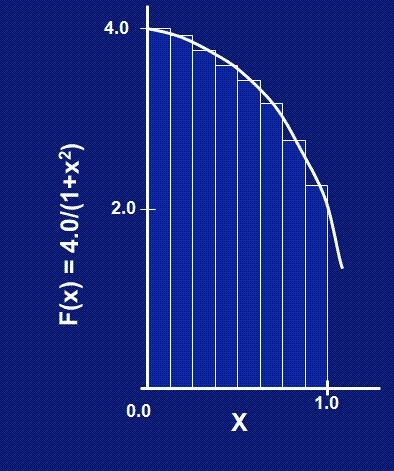
\includegraphics[width=4cm]{./pi}
    \end{center}
  \end{columns}

  \begin{algorithm}[H]
    \caption{Pseudo Code for Calculating Pi}
    \begin{algorithmic}
        \Function{calculate\_pi}{}
        \State $step \gets 1/n$
        \State $sum \gets 0$
        \Do{$i \gets 0\cdots n$}
        \State $x \gets (i+0.5)*step; sum \gets sum + 4/(1+x^2)$
        \EndDo
        \State $pi \gets sum * step$
        \EndFunction
    \end{algorithmic}
  \end{algorithm}
\end{frame}


\begin{frame}{SAXPY}
  \begin{itemize}
    \item SAXPY is a common operation in computations with vector processors included as part of the BLAS routines
    \item[] $y\leftarrow \alpha x + y$
%    \item SAXPY is a combination of scalar multiplication and vector addition
    \item Write a SAXPY code to multiply a vector with a scalar.
  \end{itemize}
  \begin{algorithm}[H]
    \caption{Pseudo Code for SAXPY}
    \begin{algorithmic}
      \Program{saxpy}{}
      \State $n \gets$ some large number
      \State $x(1:n) \gets$ some number say, 1
      \State $y(1:n) \gets$ some other number say, 2
      \State $a \gets$ some other number ,say, 3
      \Do{$i \gets 1\cdots n$}
      \State $y_i \gets y_i + a * x_i$
      \EndDo
      \EndProgram{saxpy}
    \end{algorithmic}
  \end{algorithm}
\end{frame}

\begin{frame}[allowframebreaks]{Matrix Multiplication}
  \begin{itemize}
    \item Most Computational code involve matrix operations such as matrix multiplication.
    \item Consider a matrix {\bf C} which is a product of two matrices {\bf A} and {\bf B}:
    \item[] Element {\it i,j} of {\bf C} is the dot product of the $i^{th}$ row of {\bf A} and $j^{th}$ column of {\bf B}
    \item Write a MATMUL code to multiple two matrices.
  \end{itemize}
  \begin{center}
    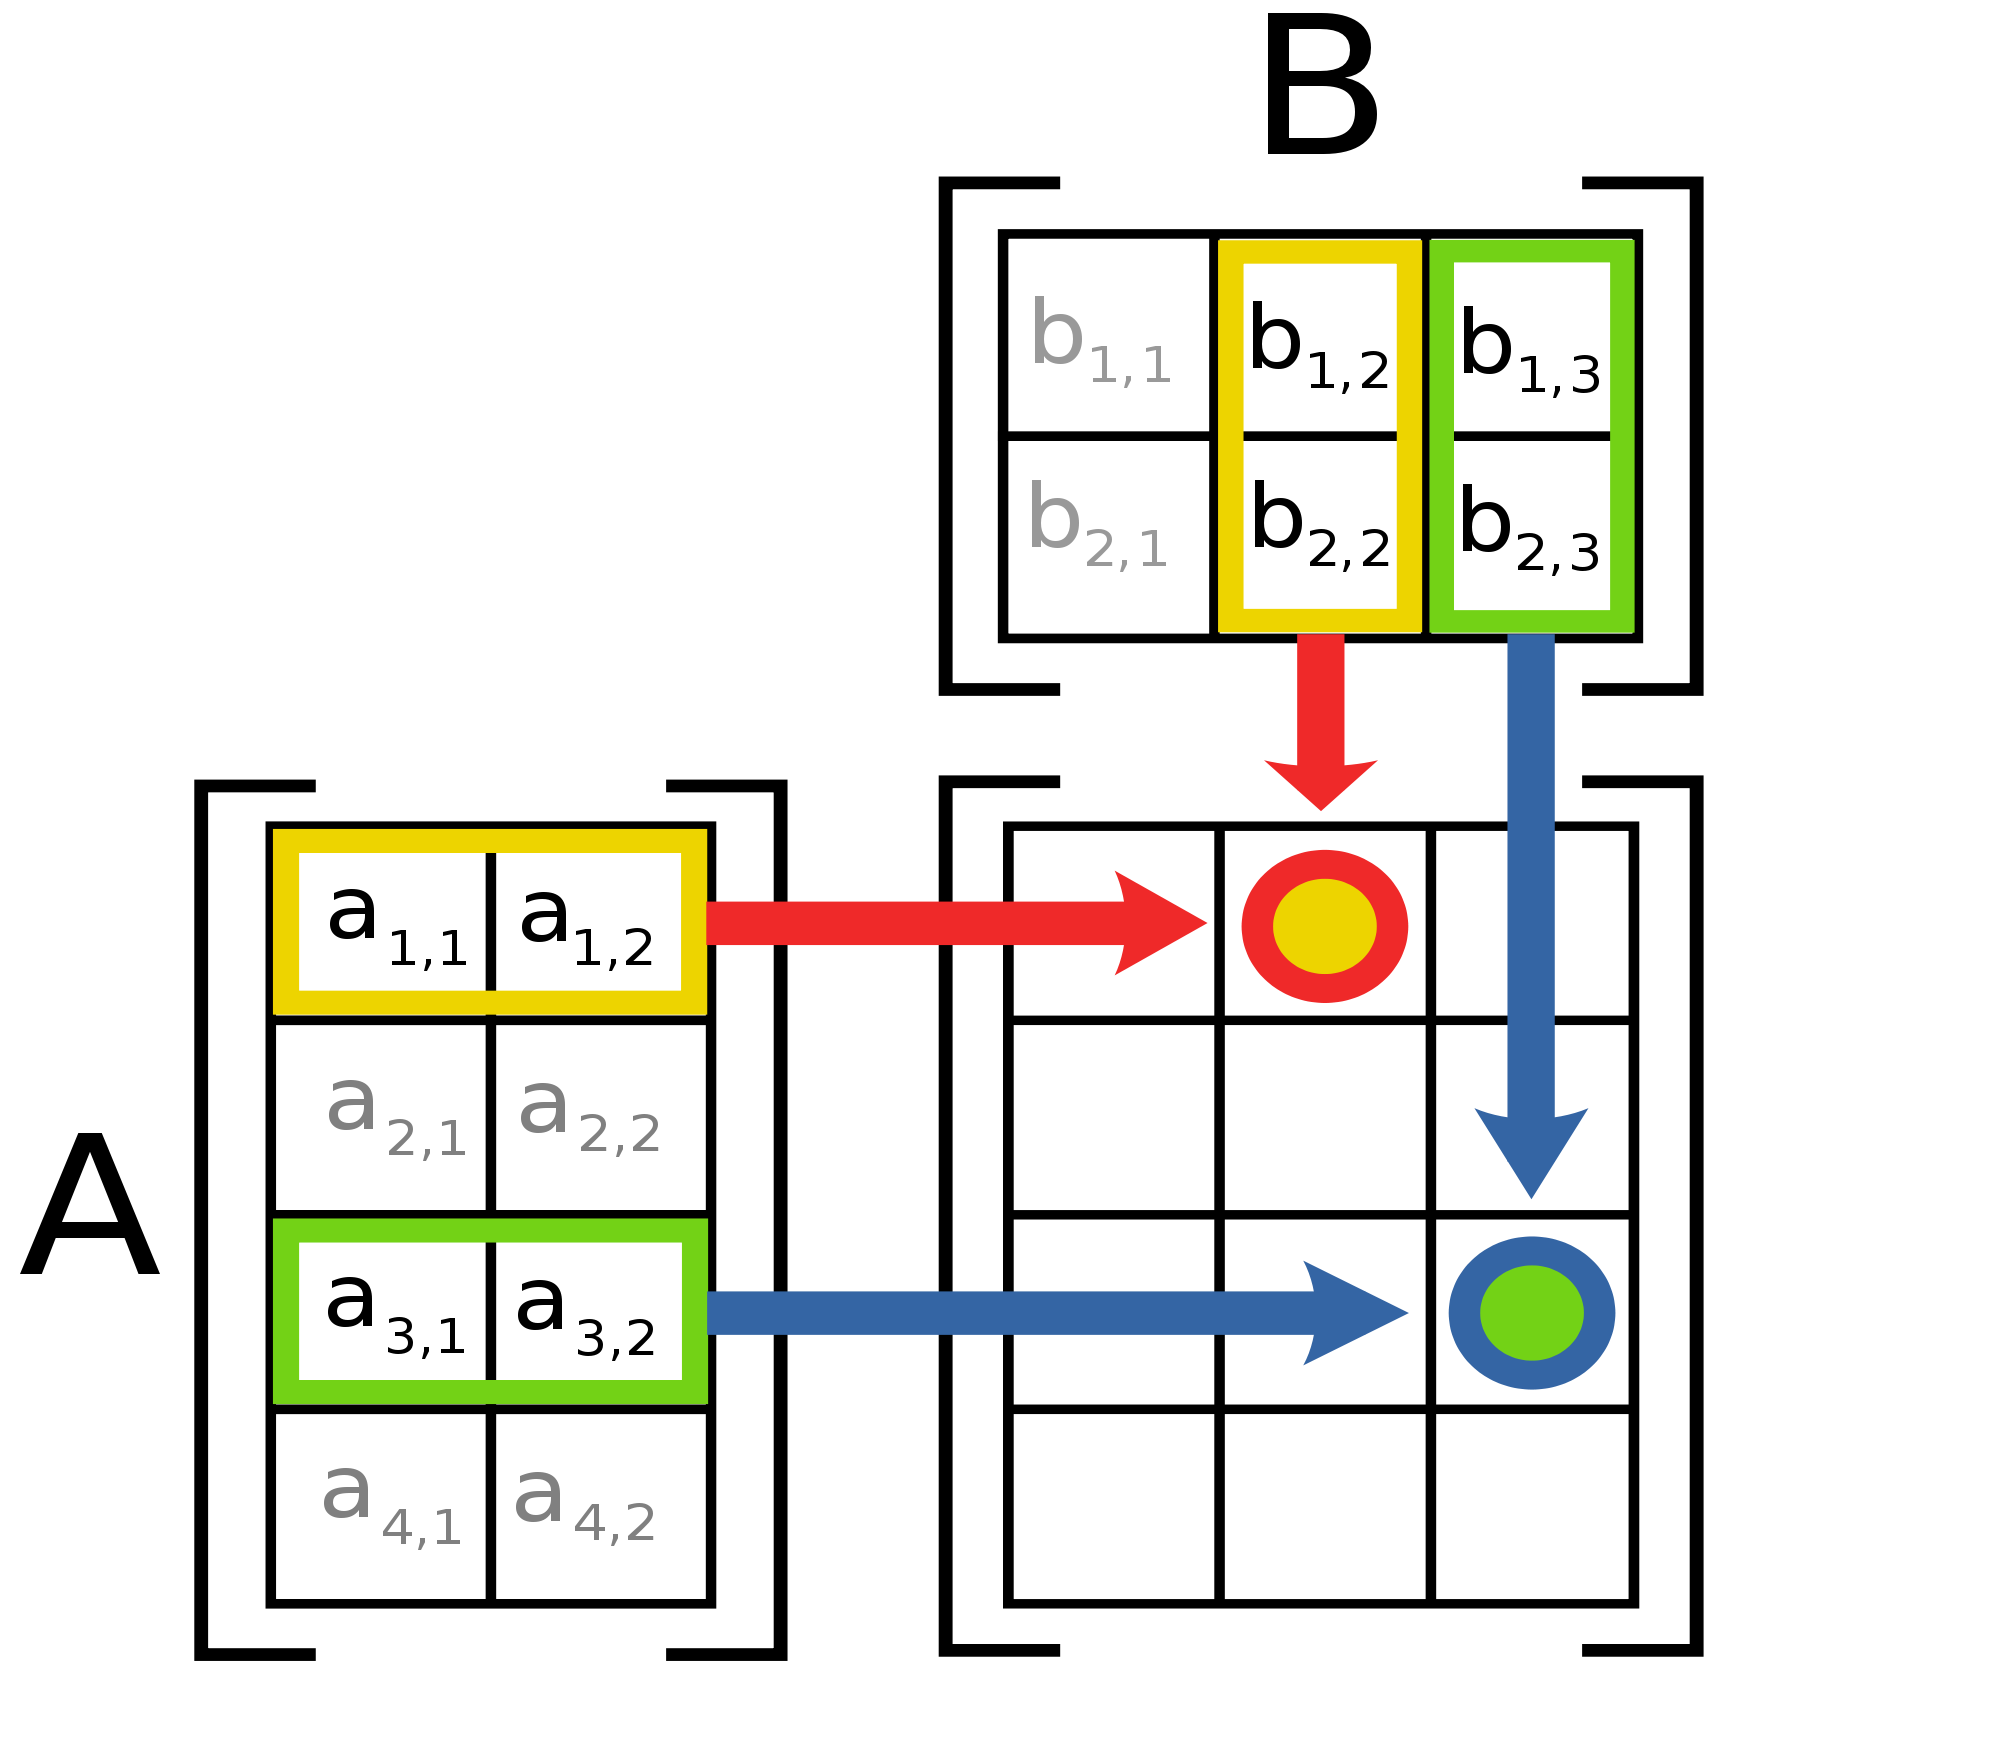
\includegraphics[width=0.3\textwidth]{./matmul}
  \end{center}

  \begin{algorithm}[H]
    \caption{Pseudo Code for MATMUL}
    \begin{algorithmic}
      \Program{matmul}{}
      \State $m,n \gets$ some\,large\,number $\le 1000$
      \State Define $a_{mn}, b_{nm}, c_{mm}$
      \State $a_{ij} \gets i+j; b_{ij} \gets i-j; c_{ij} \gets 0$
      \Do{$i \gets 1\cdots m$}
      \Do{$j \gets 1\cdots m$}
      \State $c_{i,j} \gets \sum^{n}_{k=1} a_{i,k}*b_{k,j}$
      \EndDo
      \EndDo
      \EndProgram{matmul}
    \end{algorithmic}
  \end{algorithm}
\end{frame}

\end{document}
